
\documentclass[nooutcomes]{ximera}
%\documentclass[space,handout,nooutcomes]{ximera}

% For preamble materials

\usepackage{pgf,tikz}
\usepackage{mathrsfs}
\usetikzlibrary{arrows}
\usepackage{framed}
\usepackage{amsmath}
%\pgfplotsset{compat=1.16}

\graphicspath{
  {./}
  {algorithms/}
  {../algorithms/}
}

\pdfOnly{\renewenvironment{image}[1][]{\begin{center}}{\end{center}}}

%%% This set of code is all of our user defined commands
\newcommand{\bysame}{\mbox{\rule{3em}{.4pt}}\,}
\newcommand{\N}{\mathbb N}
\newcommand{\C}{\mathbb C}
\newcommand{\W}{\mathbb W}
\newcommand{\Z}{\mathbb Z}
\newcommand{\Q}{\mathbb Q}
\newcommand{\R}{\mathbb R}
\newcommand{\A}{\mathbb A}
\newcommand{\D}{\mathcal D}
\newcommand{\F}{\mathcal F}
\newcommand{\ph}{\varphi}
\newcommand{\ep}{\varepsilon}
\newcommand{\aph}{\alpha}
\newcommand{\QM}{\begin{center}{\huge\textbf{?}}\end{center}}

\renewcommand{\le}{\leqslant}
\renewcommand{\ge}{\geqslant}
\renewcommand{\a}{\wedge}
\renewcommand{\v}{\vee}
\renewcommand{\l}{\ell}
\newcommand{\mat}{\mathsf}
\renewcommand{\vec}{\mathbf}
\renewcommand{\subset}{\subseteq}
\renewcommand{\supset}{\supseteq}
\renewcommand{\emptyset}{\varnothing}
\newcommand{\xto}{\xrightarrow}
\renewcommand{\qedsymbol}{$\blacksquare$}
\newcommand{\bibname}{References and Further Reading}
\renewcommand{\bar}{\protect\overline}
\renewcommand{\hat}{\protect\widehat}
\renewcommand{\tilde}{\widetilde}
\newcommand{\tri}{\triangle}
\newcommand{\minipad}{\vspace{1ex}}
\newcommand{\leftexp}[2]{{\vphantom{#2}}^{#1}{#2}}

%% More user defined commands
\renewcommand{\epsilon}{\varepsilon}
\renewcommand{\theta}{\vartheta} %% only for kmath
\renewcommand{\l}{\ell}
\renewcommand{\d}{\, d}
\newcommand{\ddx}{\frac{d}{dx}}
\newcommand{\dydx}{\frac{dy}{dx}}


\usepackage{bigstrut}


\newenvironment{sectionOutcomes}{}{}

\usepackage{array}
%\setlength{\extrarowheight}{-.2cm}   % Commented out by Findell to fix table headings.  Was this for typesetting division?  
\newdimen\digitwidth
\settowidth\digitwidth{9}
\def~{\hspace{\digitwidth}}
\def\divrule#1#2{
\noalign{\moveright#1\digitwidth
\vbox{\hrule width#2\digitwidth}}}


\title{Dividing Fractions}
\author{Bart Snapp and Brad Findell and Jenny Sheldon}
\begin{document}
\begin{abstract}
Problems about division and rational numbers.
\end{abstract}
\maketitle


%\begin{problem}
%Problem
%\begin{freeResponse}
%\begin{hint}
%Hint
%\end{hint}
%\end{freeResponse}
%\end{problem} 

\begin{problem}
{\em I have a recipe which calls for $4$ cups of flour.  If I make $\frac{1}{3}$ of a batch, how many cups of flour will I use?}

Which type of division is the above problem?
\begin{multipleChoice}
	\choice{The problem is a how many groups division problem.}
	\choice{The problem is a how many in one group division problem.}
	\choice[correct]{The problem is not a division problem.}
\end{multipleChoice}
\end{problem}



\begin{problem}
{\em I have a recipe which calls for $6$ cups of flour.  If I use $\frac{7}{5}$ of a cup of flour, how many batches can I make?}

Which type of division is the above problem?
\begin{multipleChoice}
	\choice[correct]{The problem is a how many groups division problem.}
	\choice{The problem is a how many in one group division problem.}
	\choice{The problem is not a division problem.}
\end{multipleChoice}
\end{problem}



\begin{problem}
{\em We know that $\frac{7}{12}$ of a cup of water fills $\frac{3}{8}$ of a jug.  How much water will fill the whole jug?}

Which type of division is the above problem?
\begin{multipleChoice}
	\choice{The problem is a how many groups division problem.}
	\choice[correct]{The problem is a how many in one group division problem.}
	\choice{The problem is not a division problem.}
\end{multipleChoice}
\end{problem}


\begin{problem}
{\em We know that $\frac{7}{12}$ of a cup of water fills $\frac{3}{8}$ of a jug.  If we pour $\frac{1}{2}$ of a cup of water into the jug, how many more cups can I add later?}

Which type of division is the above problem?
\begin{multipleChoice}
	\choice{The problem is a how many groups division problem.}
	\choice{The problem is a how many in one group division problem.}
	\choice[correct]{The problem is not a division problem.}
\end{multipleChoice}
\end{problem}



\begin{problem}
Petra is working on the following division problem.

{\em My grandma's favorite cookie recipe calls for $1 \frac{1}{3}$ cups of chocolate chips.  If I have $3$ cups of chocolate chips, how many batches can I make?}

To solve the problem, Petra draws the following picture.
\begin{center}
	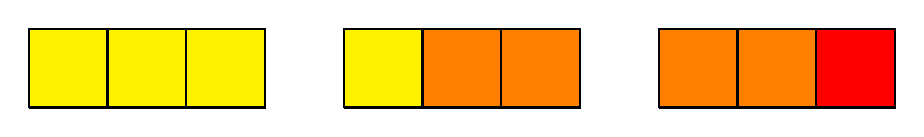
\begin{tikzpicture}
		\draw[thick, fill=yellow] (0,0)--(3,0)--(3,1)--(0,1)--(0,0);
		\draw[thick, fill=yellow] (4,0)--(5,0)--(5,1)--(4,1)--(4,0);
		\draw[thick, fill=orange] (5,0)--(7,0)--(7,1)--(5,1)--(5,0);
		\draw[thick, fill=orange] (8,0)--(10,0)--(10,1)--(8,1)--(8,0);
		\draw[thick, fill=red] (10,0)--(11,0)--(11,1)--(10,1)--(10,0);
		\draw[thick] (1,0)--(1,1);
		\draw[thick] (2,0)--(2,1);
		\draw[thick] (6,0)--(6,1);
		\draw[thick] (9,0)--(9,1);
	\end{tikzpicture}
\end{center}

Petra says, ``The yellow shaded region is one batch, and the orange shaded region is another batch.  Then we have just the red box left, so the answer is $2 \frac{1}{3}$.''  Is Petra correct?  Explain either why she is correct or where she has gone wrong.

\begin{freeResponse}
	\begin{hint}
	Petra is not correct.  She has correctly highlighted the two full batches, but her answer should be a number of batches, not a number of cups.  The red box is $\frac{1}{3}$ of a cup (since we see the cup cut into three equal pieces), but she should recognize that the batch is made out of four copies of one of these boxes.  So, the red shaded area is $\frac{1}{4}$ of a batch, so the answer is $2 \frac{1}{4}$ batches of cookies.
	\end{hint}
\end{freeResponse} 


\end{problem}




\begin{problem}
A neighborhood watch committee patrols a route which is $\frac{18}{5}$ of a mile long.  If Mrs. Little walks $\frac{2}{3}$ of a mile each day along the route, what fraction of the route is Mrs. Little patrolling?

What type of division is this?  Then, use a picture to answer this problem.

\begin{prompt}
	This is a \wordChoice{\choice[correct]{how many groups}\choice{how many in each group}} problem.  Mrs. Little patrols $\answer{\frac{5}{27}}$ of the route.
\end{prompt}
\end{problem}



\begin{problem}
Lin bought $\frac{9}{4}$ of a pound of almond flour at the grocery yesterday.  If she spent $\frac{11}{3}$ of a dollar, how much was almond flour per pound?

What type of division is this?  Then, use a picture to answer this problem.

\begin{prompt}
This is a \wordChoice{\choice{how many groups}\choice[correct]{how many in each group}} problem.  Almond flour was $\answer{\frac{44}{27}}$ of a dollar per pound.
\end{prompt}

\end{problem}



\end{document}



